% Copyright 2006 by Till Tantau
%
% This file may be distributed and/or modified
%
% 1. under the LaTeX Project Public License and/or
% 2. under the GNU Free Documentation License.
%
% See the file doc/generic/pgf/licenses/LICENSE for more details.


\section{Spy Library: Magnifying Parts of Pictures}
\label{section-library-spy}

\begin{tikzlibrary}{spy}
    The package defines options for creating pictures in which some part of the
    picture is repeated in another area in a magnified way (as if you were
    looking through a spyglass, hence the name).
\end{tikzlibrary}
%
\begin{codeexample}[setup code,hidden]
    \usetikzlibrary{decorations.fractals,spy}
\end{codeexample}


\subsection{Magnifying a Part of a Picture}

The idea behind the |spy| library is to make is easy to create high-density
pictures in which some important parts are repeated somewhere, but magnified as
if you were looking through a spyglass:
%
\begin{codeexample}[]
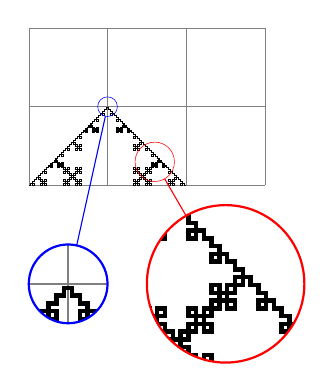
\begin{tikzpicture}
  [spy using outlines={circle, magnification=4, size=2cm, connect spies}]

  \draw [help lines] (0,0) grid (3,2);

  \draw [decoration=Koch curve type 1]
    decorate { decorate{ decorate{ decorate{ (0,0) -- (2,0) }}}};

  \spy [red] on (1.6,0.3)
             in node [left] at (3.5,-1.25);

  \spy [blue, size=1cm] on (1,1)
              in node [right] at (0,-1.25);
\end{tikzpicture}
\end{codeexample}

\begin{codeexample}[]
\begin{tikzpicture}[spy using overlays={size=12mm}]
  \draw [decoration=Koch snowflake]
    decorate { decorate{ decorate{ decorate{ (0,0) -- (2,0) }}}};

  \spy [green,magnification=3] on (0.6,0.1) in node at (-0.3,-1);
  \spy [blue,magnification=5]  on (1,0.5)   in node at (1,-1);
  \spy [red,magnification=10]  on (1.6,0.1) in node at (2.3,-1);
\end{tikzpicture}
\end{codeexample}

Note that this magnification uses what is called a \emph{canvas transformation}
in this manual: Everything is magnified, including line width and text.

In order for ``spying'' to work, the picture obviously has to be drawn several
times: Once at its normal size and then again for each ``magnifying glass''.
Several keys and commands work in concert to make this possible:
%
\begin{itemize}
    \item You need to make \tikzname\ aware of the fact that a picture (or just
        a scope) is to be magnified. This is done by adding the special key
        |spy scope| to a |{scope}| or |{tikzpicture}| (which is also just a
        scope). Some special keys like |spy using outlines| implicitly set the
        |spy scope|.
    \item Inside this scope you may then use the command |\spy|, which is only
        available inside such scopes (so there is no danger of you
        inadvertently using this command outside such a scope). This command
        has a special syntax and will (at some point) create two nodes: One
        node that shows the magnified picture (called the \emph{spy-in node})
        and another node showing which part of the original picture is
        magnified (called the \emph{spy-on} node). The spy-in node is, indeed,
        a normal node, so it can have any shape or border that you like and you
        can apply all of \tikzname's advanced features to it. The only
        difference compared to a normal node is that instead of some ``text''
        it contains a magnified version of the picture, clipped to the size of
        the node.

        The |\spy| command does not create the nodes immediately. Rather, the
        creation of these nodes is postponed till the end of the |spy scope| in
        which the |\spy| command is used. This is necessary since in order to
        repeat the whole scope inside the node containing the magnified
        version, the whole picture needs to be available when this node is
        created.
\end{itemize}

A basic question any library for ``magnifying things'' has to address is how
you specify which part of the picture is to be magnified (the spy-on node) and
where this magnified part is to be shown (the spy-in node). There are two
possible ways:
%
\begin{enumerate}
    \item You specify the size and position of the spy-on node. Then the size
        of the spy-in node is determined by the size of the spy-on node and the
        magnification factor -- you can still decide where the spy-in node
        should be placed, but not its size.
    \item Alternatively, you specify the size and position of the spy-in node.
        Then, similarly to the first case, the size of the spy-on node is
        determined implicitly and you can only decide where the spy-on node
        should be placed, but not its size.
\end{enumerate}

The |spy| library uses the second method: You specify the size and position of
the spy-in nodes, the sizes of the spy-on nodes are then computed
automatically.


\subsection{Spy Scopes}

\begin{key}{/tikz/spy scope=\meta{options} (default \normalfont empty)}
    This option may be used with a |{scope}| or any environment that creates
    such a scope internally (like |{tikzpicture}|). It has the following
    effects:
    %
    \begin{itemize}
        \item It resets a number of graphic state parameters, including the
            color, line style, and others. This is necessary for technical
            reasons.
        \item It tells \tikzname\ that the content of the scope should be saved
            internally in a special box.
        \item It defines the command |\spy| so that it can be used inside the
            scope.
        \item At the end of the scope, the nodes belonging to the |\spy|
            commands used inside the scope are created.
        \item The \meta{options} are saved in an internal style. Each time
            |\spy| is used, these \meta{options} will be used.
        \item Three keys are defined that provide useful shortcuts:
            %
            \begin{key}{/tikz/size=\meta{dimension}}
                Inside a |spy scope|, this is a shortcut for |minimum size|.
            \end{key}
            %
            \begin{key}{/tikz/height=\meta{dimension}}
                Inside a |spy scope|, this is a shortcut for |minimum height|.
            \end{key}
            %
            \begin{key}{/tikz/width=\meta{dimension}}
                Inside a |spy scope|, this is a shortcut for |minimum width|.
            \end{key}
    \end{itemize}
    %
    It is permissible to nest |spy scopes|. In this case, all |\spy| commands
    inside the inner |spy scope| only have an effect on material inside the
    scope, whereas |\spy| commands outside the inner |spy scope| but inside the
    outer |spy scope| allow you to ``spy on the spy''.
    %
\begin{codeexample}[]
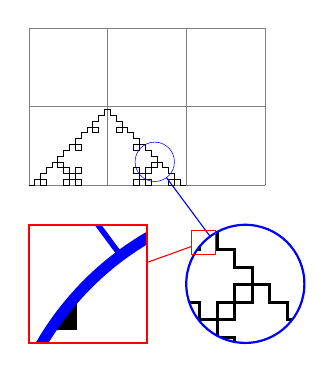
\begin{tikzpicture}
  [spy using outlines={rectangle, red, magnification=5,
                       size=1.5cm, connect spies}]

  \begin{scope}
    [spy using outlines={circle, blue,
                         magnification=3, size=1.5cm, connect spies}]
    \draw [help lines] (0,0) grid (3,2);

    \draw [decoration=Koch curve type 1]
      decorate{ decorate{ decorate{ (0,0) -- (2,0) }}};

    \spy on (1.6,0.3) in node (zoom) [left] at (3.5,-1.25);
  \end{scope}

  \spy on (zoom.north west) in node [right] at (0,-1.25);
\end{tikzpicture}
\end{codeexample}
    %
\end{key}


\subsection{The Spy Command}

\begin{command}{\spy \opt{\oarg{options}} |on| \meta{coordinate} \texttt{in node} \meta{node options}|;|}
    This command can only be used inside a |spy scope|. Let us start with the
    syntax:
    %
    \begin{itemize}
        \item The |\spy| command is not a special case of |\path|. Rather, it
            has a small parser of its own.
        \item Following the optional \meta{options}, you must write |on|,
            followed by a coordinate. This coordinate will be the center of the
            area that is to be magnified.
        \item Following the \meta{coordinate}, you must write |in node|
            followed by some \meta{node options}. The syntax for these options
            is the same as for a normal |node| path command, such as |[left]|
            or |(foo) [red] at (bar)|. \emph{However}, \meta{node options} are
            \emph{not} followed by a curly brace. Rather, the \meta{node
            options} must directly be followed by a semicolon.
    \end{itemize}
    %
    The effect of this command is the following: The \meta{options},
    \meta{coordinate}, and \meta{node options} are stored internally till the
    end of the current |spy scope|. This means that, in particular, you can
    reference any node inside the |spy scope|, even if it is not yet defined
    when the |\spy| command is given. At the end of the current |spy scope|,
    two nodes are created, called the \emph{spy-in node} and the \emph{spy-on
    node}.
    %
    \begin{itemize}
        \item The \emph{spy-in node} is the node that contains a magnified part
            of the picture (the node \emph{in} which we see on what we spy).
            This node is, indeed, a normal \tikzname\ node, so you can use all
            standard options to style this node. In particular, you can specify
            a shape or a border color or a drop shadow or whatever. The only
            thing that is special about this node is that instead of containing
            some normal text, its ``text'' is the magnified picture.

            To be precise, the picture of the |spy scope| is scaled by a
            certain factor, specified by the |lens| or |magnification| options
            discussed below, and is shifted in such a way that the
            \meta{coordinate} lies at the center of the spy-on node.
        \item The \emph{spy-on node} is a node that is centered on the
            \meta{coordinate} and whose size reflects exactly the area shown
            inside the spy-in node (the node containing \emph{on} what we spy).
    \end{itemize}

    Let us now go over what happens in detail when the two nodes are
    created:
    %
    \begin{enumerate}
        \item A scope is started. Two sets of options are used with this scope:
            First, the options passed to the enclosing |spy scope| and then the
            \meta{options} (which will, thus, overrule the options of the
            |spy scope|).
        \item Then, the spy-on node is created. However, we will first discuss
            the spy-in node.
        \item The spy-in node is created after the spy-on node (and, hence,
            will cover the spy-on node in case they overlap). When this node is
            created, the \meta{node options} are used in addition to the effect
            caused by the \meta{options} and the options of the |{spy scope}|.
            Additionally, the following style is used:
            %
            \begin{stylekey}{/tikz/every spy in node}
                This style is used with every spy-in node.
            \end{stylekey}
            %
            The position of the node (the |at| option) is set to the
            \meta{coordinate} by default, so that it will cover the
            to-be-magnified area. You can change this by providing the |at|
            option yourself:
            %
\begin{codeexample}[]
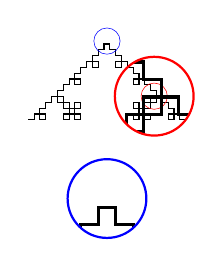
\begin{tikzpicture}
  [spy using outlines={circle, magnification=3, size=1cm}]

  \draw [decoration=Koch curve type 1]
    decorate{ decorate{ decorate{ (0,0) -- (2,0) }}};

  \spy [red]  on (1.6,0.3) in node;
  \spy [blue] on (1,1)     in node at (1,-1);
\end{tikzpicture}
\end{codeexample}
            %
            No ``text'' can be specified for the node. Rather, the ``text''
            shown inside this node is the picture of the current |spy scope|,
            but canvas-transformed according to the following key:
            %
            \begin{key}{/tikz/lens=\meta{options}}
                The \meta{options} should contain transformation commands like
                |scale| or |rotate|. These transformations are applied to the
                picture when it is shown inside the spy-on node.
            \end{key}
            %
            Since the most common transformation is undoubtedly a simple
            scaling, there is a special style for this:
            %
            \begin{key}{/tikz/magnification=\meta{number}}
                This has the same effect as saying
                |lens={scale=|\meta{number}|}|.
            \end{key}
            %
            Now, usually the size of a node is determined in such a way that it
            ``fits'' around the text of the node. For a spy-on node this is not
            a good approach since the ``text'' of this node would contain ``the
            whole picture''. Because of this, \tikzname\ acts as if the
            ``text'' of the node has zero size. You must then use keys like
            |minimum size| to cause the node to have a certain size. Note that
            the key |size| is an abbreviation for |minimum size| inside a spy
            scope.

            You can name the spy-on node in the usual ways. Additionally, the
            node is (also) always named |tikzspyinnode|. Following the spy
            scope, you can use this node like any other node:
            %
\begin{codeexample}[]
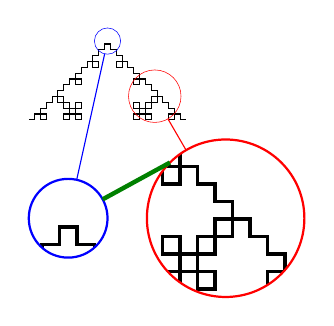
\begin{tikzpicture}
  \begin{scope}
    [spy using outlines={circle, magnification=3, size=2cm, connect spies}]

    \draw [decoration=Koch curve type 1]
      decorate{ decorate{ decorate{ (0,0) -- (2,0) }}};

    \spy [red] on (1.6,0.3) in node (a) [left] at (3.5,-1.25);

    \spy [blue, size=1cm] on (1,1) in node (b) [right] at (0,-1.25);
  \end{scope}
  \draw [ultra thick, green!50!black] (b) -- (a.north west);
\end{tikzpicture}
\end{codeexample}
            %
        \item Once both nodes have been created, the current value of the
            following key is used to connect them:
            %
            \begin{key}{/tikz/spy connection path=\meta{code} (initially \normalfont empty)}
                The \meta{code} is executed after the spy-on and spy-in nodes
                have just been created. Inside this \meta{code}, the two nodes
                can be accessed as |tikzspyinnode| and  |tikzspyonnode|. For
                example, the key |connect spies| sets this command to
                %
\begin{codeexample}[code only]
\draw[thin] (tikzspyonnode) -- (tikzspyinnode);
\end{codeexample}
            \end{key}
    \end{enumerate}
    %
    Returning to the creation of the spy-in node: This node is centered on
    \meta{coordinate} (more precisely, its anchor is set to |center| and the
    |at| option is set to \meta{coordinate}). Its size and shape are initially
    determined in the same way as the size and shape of the spy-on node
    (unless, of course, you explicitly provide a different shape for, say, the
    spy-on node locally, which is not really a good idea). Then, additionally,
    the \emph{inverted} transformation done by the |lens| option is applied,
    resulting in a node whose size and shape exactly corresponds to the area in
    the picture that is shown in the spy-on node.
    %
\begin{codeexample}[]
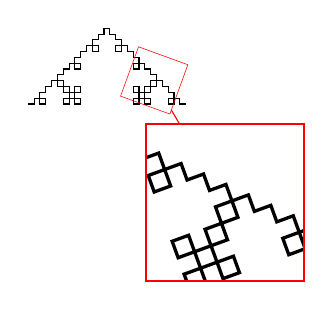
\begin{tikzpicture}
  [spy using outlines={lens={scale=3,rotate=20}, size=2cm, connect spies}]

  \draw [decoration=Koch curve type 1]
    decorate{ decorate{ decorate{ (0,0) -- (2,0) }}};

  \spy [red] on (1.6,0.3) in node at (2.5,-1.25);
\end{tikzpicture}
\end{codeexample}

    Like for the spy-in node, a style can be used to format the spy-on node:
    %
    \begin{stylekey}{/tikz/every spy on node}
        This style is used with every spy-on node.
    \end{stylekey}
    %
    The spy-on node is named |tikzspyonnode| (but, as always, this node is only
    available after the spy scope). If you have multiple spy-on nodes and you
    would like to access all of them, you need to use the |name| key inside the
    |every spy on node| style.

    The |inner sep| and |outer sep| of both spy-in and spy-on nodes are set to
    |0pt|.
\end{command}


\subsection{Predefined Spy Styles}

There are some predefined styles that make using the |spy| library easier. The
following two styles can be used instead of |spy scope|, they pass their
\meta{options} directly to |spy scope|. They additionally set up the graphic
styles to be used for the spy-in nodes and the spy-on nodes in some special
way.

\begin{key}{/tikz/spy using outlines=\meta{options} (default \normalfont empty)}
    This key creates a |spy scope| in which the spy-in node is drawn, but not
    filled, using a thick line; and the spy-on node is drawn, but not filled,
    using a very thin line.
    %
\begin{codeexample}[]
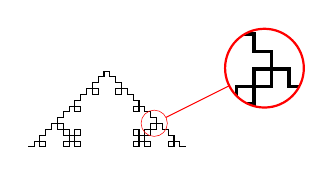
\begin{tikzpicture}
  [spy using outlines={circle, magnification=3, size=1cm, connect spies}]

  \draw [decoration=Koch curve type 1]
    decorate{ decorate{ decorate{ (0,0) -- (2,0) }}};

  \spy [red] on (1.6,0.3) in node at (3,1);
\end{tikzpicture}
\end{codeexample}
    %
\end{key}

\begin{key}{/tikz/spy using overlays=\meta{options} (default \normalfont empty)}
    This key creates a |spy scope| in which both the spy-in and spy-on nodes
    are filled, but with the fill opacity set to 20\%.
    %
\begin{codeexample}[]
\begin{tikzpicture}
  [spy using overlays={circle, magnification=3, size=1cm, connect spies}]

  \draw [decoration=Koch curve type 1]
    decorate{ decorate{ decorate{ (0,0) -- (2,0) }}};

  \spy [green] on (1.6,0.3) in node at (3,1);
\end{tikzpicture}
\end{codeexample}
    %
\end{key}

The following style is useful for connecting the spy-in and the spy-on nodes:

\begin{key}{/tikz/connect spies}
    Causes the spy-in and the spy-on nodes to be connected by a thin line.
    %
\begin{codeexample}[]
\begin{tikzpicture}
  [spy using overlays={circle, magnification=3, size=1cm}]

  \draw [decoration=Koch curve type 2]
    decorate{ decorate{ decorate{ (0,0) -- (2,0) }}};

  \spy [green] on (1.6,0.1) in node at (3,1);
  \spy [red,connect spies] on (0.5,0.4) in node at (1,1.5);
\end{tikzpicture}
\end{codeexample}
    %
\end{key}


\subsection{Examples}

Usually, the spy-in node and the spy-on node should have the same shape.
However, you might also wish to use the |circle| shape for the spy-on node and
the |magnifying glass| shape for the spy-in node:
%
\begin{codeexample}[]
\tikzset{spy using mag glass/.style={
    spy scope={
      every spy on node/.style={
        circle,
        fill, fill opacity=0.2, text opacity=1},
      every spy in node/.style={
        magnifying glass, circular drop shadow,
        fill=white, draw, ultra thick, cap=round},
      #1
    }}}
\begin{tikzpicture}[spy using mag glass={magnification=3, size=1cm}]
  \draw [decoration=Koch curve type 2]
    decorate{ decorate{ decorate{ (0,0) -- (2,0) }}};

  \spy [green!50!black] on (1.6,0.1) in node at (2.5,-0.5);
\end{tikzpicture}
\end{codeexample}

With the magnifying glass, you can also put it ``on top'' of the picture
itself:
%
\begin{codeexample}[]
\begin{tikzpicture}
  [spy scope={magnification=4, size=1cm},
   every spy in node/.style={
     magnifying glass, circular drop shadow,
     fill=white, draw, ultra thick, cap=round}]

  \draw [decoration=Koch curve type 2]
    decorate{ decorate{ decorate{ (0,0) -- (2,0) }}};

  \spy on (1.6,0.1) in node;
\end{tikzpicture}
\end{codeexample}


%%% Local Variables:
%%% mode: latex
%%% TeX-master: "pgfmanual-pdftex-version"
%%% End:
